\documentclass[a4paper,10pt]{article}
\usepackage[utf8]{inputenc}
\usepackage{amsmath}
\usepackage{xfrac}
\usepackage{float}
\usepackage[a4paper, total={7.5in, 10in}]{geometry}
\usepackage{longtable}
\usepackage[table]{xcolor}
\usepackage{listings}
\lstset{
breaklines=true
}
%http://tex.stackexchange.com/questions/116534/lstlisting-line-wrapping
\usepackage{hyperref}
\hypersetup{
    colorlinks=true,
    linkcolor=blue,
    citecolor=blue
}
\usepackage{color}
 
\definecolor{codegreen}{rgb}{0,0.6,0}
\definecolor{codegray}{rgb}{0.5,0.5,0.5}
\definecolor{codepurple}{rgb}{0.58,0,0.82}
\definecolor{backcolour}{rgb}{0.95,0.95,0.92}
 
\lstdefinestyle{mystyle}{
    backgroundcolor=\color{backcolour},   
    commentstyle=\color{codegreen},
    keywordstyle=\color{magenta},
    numberstyle=\tiny\color{codegray},
    stringstyle=\color{codepurple},
    basicstyle=\footnotesize,
    breakatwhitespace=false,         
    breaklines=true,                 
    captionpos=b,                    
    keepspaces=true,                 
    numbers=left,                    
    numbersep=5pt,                  
    showspaces=false,                
    showstringspaces=false,
    showtabs=false,                  
    tabsize=2
}
 
\lstset{style=mystyle}

%opening

\title{}
\author{}
\date{}

\begin{document}

\section*{Python code and analysis}
\begin{lstlisting}[language=python]
import numpy as np
import matplotlib.pyplot as plt

a = 3.0               # the half width of the well in angstroms 
m = 1.0               # mass of electron in 1 me units
V0 = 10.0             # height/depth of well in eV
hbar = 1.0            # hbar
delta = np.sqrt(2.0*m*V0*(a**2.0)/(hbar**2.0))     # Defined in the hand written solution
eta = np.arange(0.001,2*np.pi,0.01)  # Defined in the hand written solutiom

def f(f,eta):
    """
    This is the lhs in the transcendental equations.
    """
    return np.sqrt(((delta/eta)**2.0)-1.0)

def f1(eta):
    """
    The equation whose zeros are to be found to obtain the even solution.
    """
    return f(eta) - np.tan(eta)

def f2(eta):
    """
    The equation whose zeros are to be found to obtain the odd solution.
    """
    return f(eta) + (1.0/np.tan(eta))

def firstDerivative_O4(function,x0,stepsize):
    """
    Returns first derivative of the function "function" at the point x0 by considering points, one and two steps on either side of x0.
    The Accuracy is of order (stepsize)^4.
    """
    return (function(x0 - 2.0*stepsize) - 8.0*function(x0 - stepsize) + 8.0*function(x0 + stepsize) - function(x0 + 2.0*stepsize))/(12.0*stepsize)

def Newton_Raphson(f,x0,stepsize):
    """
    Returns the zero of f. x0 is the guess. stepsize will be used for determining the first derivative of f.
    """
    fprime = firstDerivative_O4(f,x0,stepsize)
    x1 = x0 - (f(x0)/fprime)
    while((x0 - x1) >= stepsize**(8.0)):
        x0 = x1
        fprime = firstDerivative_O4(f,x0,stepsize)
        x1 = x0 - f(x0)/fprime
    return x1

def get_energy(eta):
    """
    Gets energy value for given eta value.
    """
    return (eta**2.0)*(hbar**2.0)/(2.0*m*(a**2.0))

##### Main portion begins #####

even_guess = np.pi/4.0   # Guess for even solution
odd_guess = 0.999*np.pi  # Guess for odd solution
even_sol = Newton_Raphson(f1,even_guess,10**(-3)) # Obtaining the solution using the Newton Raphson method
odd_sol = Newton_Raphson(f2,odd_guess,10**(-3))   # Obtaining the solution using the Newton Raphson method

### Printing the solutions
print("eta for even sol : {etev:0.6f}".format(etev=even_sol))
print("eta for odd sol : {etod:0.6f}".format(etod=odd_sol))
print("Energy for even state is : {e2:0.6f}".format(e2=get_energy(even_sol)))
print("Energy for odd state is : {e1:0.6f}".format(e1=get_energy(odd_sol)))

\end{lstlisting}

The outputs are shown below :

\begin{table}
\begin{tabular}{cccc}
Even solution & Odd solution & Even energy & Odd energy \\
1.2772178959669078 & 2.5387246419461156 & 0.09062697520989639 & 0.3580623782013574 \\
\end{tabular}
\end{table}


\begin{figure}[H]
\centering
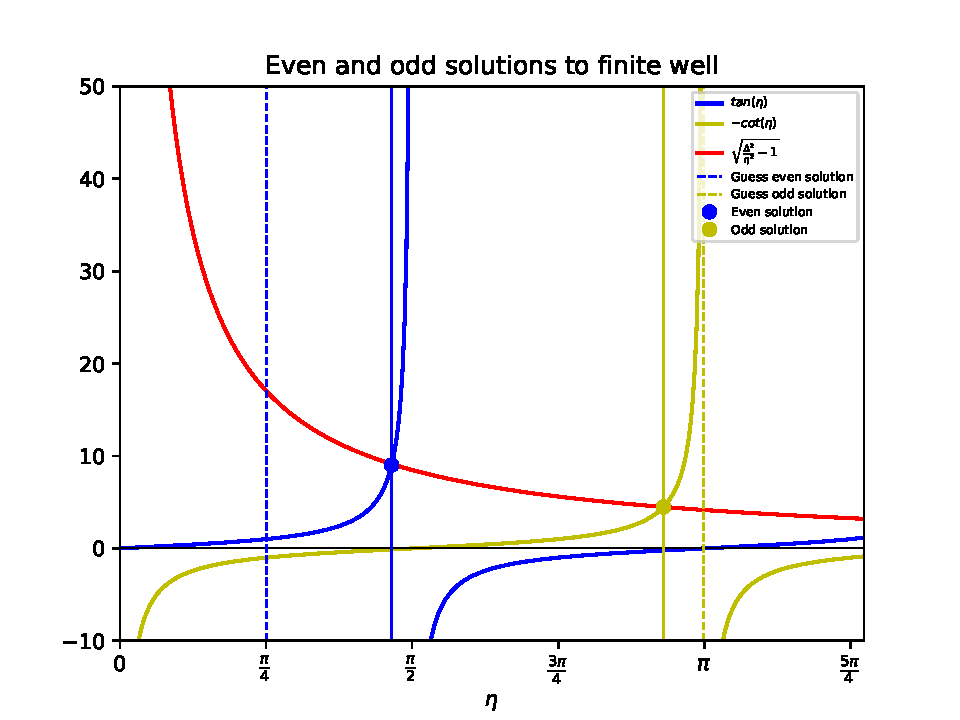
\includegraphics[scale=0.9]{transcendental_sol.pdf} 
\end{figure}

\begin{figure}[H]
\centering
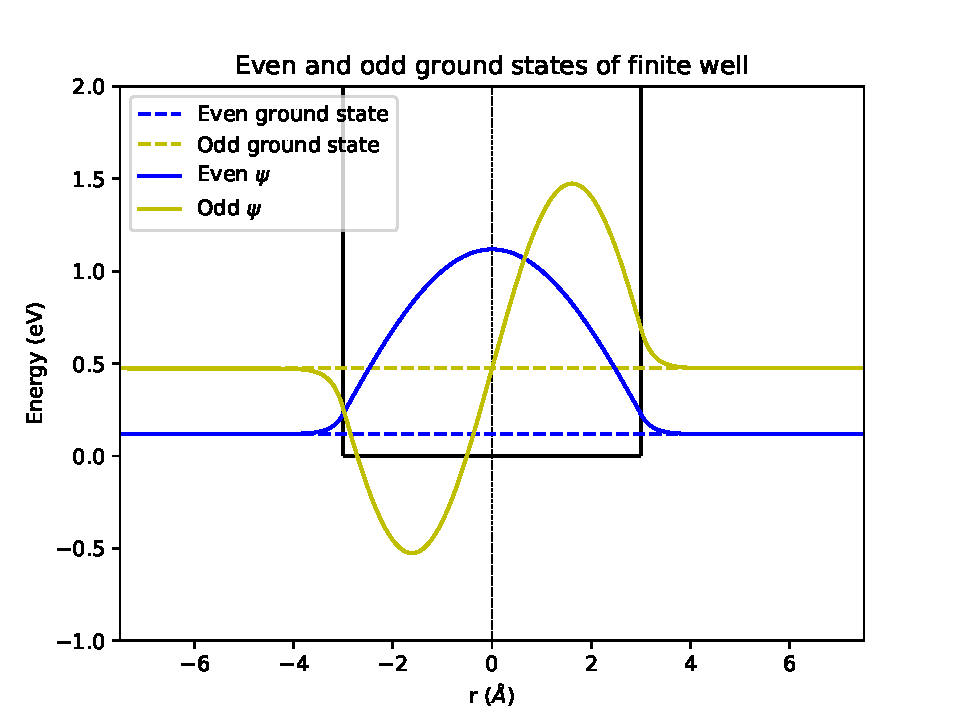
\includegraphics[scale=0.9]{wavefunction_plot_zoomed.pdf} 
\end{figure}


\end{document}
